\documentclass[11pt]{article}

\usepackage[T1]{fontenc}
\usepackage[utf8]{inputenc}
\usepackage[english]{babel}
\usepackage[margin=1in]{geometry}
\usepackage{lmodern}
\usepackage{microtype}
\usepackage{mathtools,amssymb,amsthm}
\usepackage{graphicx}
\usepackage{booktabs,tabularx,array}
\usepackage{caption}
\usepackage{enumitem}
\usepackage{fancyhdr}
\usepackage[numbers,sort&compress]{natbib}
\usepackage{orcidlink}
\usepackage{titling}
\usepackage{titlesec}
\usepackage{doi,xurl,aliascnt}
\usepackage{hyperref}
\usepackage[nameinlink,noabbrev]{cleveref}

\hypersetup{
  pdftitle={Six Birds Foundations IX: Exact Reachability for Audited Markov Edits},
  pdfauthor={Ioannis Tsiokos},
  hidelinks
}
\urlstyle{same}
\captionsetup{
  font=small,
  labelfont=bf,
  labelsep=period,
  margin=1em
}
\captionsetup[table]{skip=6pt,position=top}
\captionsetup[figure]{skip=6pt}
\setlist[enumerate]{leftmargin=*, itemsep=2pt, topsep=4pt}
\setlist[itemize]{leftmargin=*, itemsep=2pt, topsep=4pt}
\setlength{\droptitle}{-3.2em}
\pretitle{\begin{center}\LARGE\bfseries}
\posttitle{\par\end{center}\vspace{0.5em}}
\preauthor{\begin{center}\normalsize}
\postauthor{\par\end{center}\vspace{-0.4em}}
\predate{\begin{center}\small}
\postdate{\par\end{center}\vspace{0.6em}}
\setlength{\emergencystretch}{2em}
\clubpenalty=10000
\widowpenalty=10000
\displaywidowpenalty=10000
\interfootnotelinepenalty=10000
\allowdisplaybreaks[2]
\setlength{\bibsep}{2pt plus 0.3ex}

\pagestyle{fancy}
\fancyhf{}
\fancyhead[L]{\small\itshape Six Birds Foundations IX}
\fancyhead[R]{\small\thepage}
\renewcommand{\headrulewidth}{0.4pt}
\renewcommand{\footrulewidth}{0pt}

\fancypagestyle{firstpage}{%
  \fancyhf{}
  \fancyfoot[C]{\scriptsize Automorph Inc., Wilmington, DE, USA
    \quad \texttt{ioannis@automorph.io} \quad \textcopyright\ 2026
    \quad CC-BY 4.0 \quad Preprint --- not peer reviewed.}
  \renewcommand{\headrulewidth}{0pt}
  \renewcommand{\footrulewidth}{0pt}
}

\titlespacing*{\section}{0pt}{2.8ex plus 1.0ex minus 0.4ex}{1.6ex plus 0.4ex}
\titlespacing*{\subsection}{0pt}{2.2ex plus 0.8ex minus 0.3ex}{1.1ex plus 0.3ex}

\newtheorem{theorem}{Theorem}[section]
\newaliascnt{proposition}{theorem}
\newtheorem{proposition}[proposition]{Proposition}
\aliascntresetthe{proposition}
\newaliascnt{lemma}{theorem}
\newtheorem{lemma}[lemma]{Lemma}
\aliascntresetthe{lemma}
\theoremstyle{definition}
\newaliascnt{definition}{theorem}
\newtheorem{definition}[definition]{Definition}
\aliascntresetthe{definition}
\crefname{proposition}{proposition}{propositions}
\Crefname{proposition}{Proposition}{Propositions}
\crefname{lemma}{lemma}{lemmas}
\Crefname{lemma}{Lemma}{Lemmas}
\crefname{definition}{definition}{definitions}
\Crefname{definition}{Definition}{Definitions}

\newcommand{\QQ}{\mathbb{Q}}
\newcommand{\RR}{\mathbb{R}}
\newcommand{\NN}{\mathbb{N}}
\newcommand{\Core}{\operatorname{core}}
\newcommand{\SCore}{\operatorname{sc}}
\newcommand{\supp}{\operatorname{supp}}
\newcommand{\sgn}{\operatorname{sgn}}
\newcommand{\Refines}{\preceq}
\newcommand{\Norm}[1]{\left\lVert #1 \right\rVert_\infty}
\newcommand{\Fatcd}{\textsc{FATCD}}

\title{Six Birds Foundations IX:\\[4pt]
Exact Reachability for Audited Markov Edits}
\author{Ioannis Tsiokos\,\orcidlink{0009-0009-7659-5964}}
\date{Version 1: November 22, 2026}

\begin{document}
\maketitle
\thispagestyle{firstpage}
\begin{abstract}
\noindent
We characterize when a marked Markov instrument can change its stochastic
law by arbitrarily fine finite chains of rational edits while retaining
its held experimental tests. For a class with a positive parity mixture
and a conditional register, reachability is equivalent to advance in the
capability order and equality of a signed core computed from the initial
tests. The core records the least support reachable by integer damping
and the signs of its surviving coordinates. Active equations are
recomputed as coordinates vanish. We prove completeness using real chart
limits, exact rational interpolation and estimates in the metric on
prepared transition probabilities. One example requires two successive
contractions to reach the core, and another gives an obstruction at
positive tolerance. A coupled instrument realizes all six Foundations II
witnesses, and every chain connecting one pair of its states uses all
six observable effects. The declared single-write language has a
five-family minimum because one disclosure command accepts a clock
grade. A contract requiring the family name to determine whether an
invocation changes the terminal decision readout forces six families
on this instrument. The reachability, omission, family and witness
results are formalized in Lean.
\end{abstract}

\section{Introduction}\label{sec:introduction}

A description used at a higher level of a system carries commitments. It may
specify which transitions are feasible, which decisions can be made before a
deadline, which routes have equal effects, or which measured values can be cited.
Changing that description can expose new distinctions, but the changes are useful
only if the commitments already in force retain their meaning. The problem in
this paper is to decide, from two measured endpoint laws and those commitments,
whether a finite sequence of lawful edits connects the endpoints at every
positive tolerance.

Six Birds Foundations I organized changes of a description around six
roles~\citep{foundations1}. In finite Markov systems, the framework has been
used to realize stochastic packages while preserving observed
histories~\citep{finitepackaging} and to identify limits of deterministic
coarse-graining~\citep{nogo}.
Six Birds Foundations~II specifies a witness predicate for each role
and proves a classification of finite audited typed closure descriptions
under a recognition hypothesis~\citep{foundations2v3}.
Here we define lawful edits directly from a Markov instrument's measured
probabilities and named tests. \Cref{thm:native} gives an exact
reachability criterion for this model. \Cref{thm:omission,thm:basis}
then determine which measured changes a chain requires and how the
corresponding commands can be grouped. One connection requires all six
effects, and five single-write command families generate the entire edit
relation. The witness construction in \Cref{prop:witness-realization}
shows why the six effects instantiate the distinct Foundations~II roles.

\subsection{A route that releases a pinned response}\label{sec:opening-example}

Consider a two-state base with a sign probe \(\chi\) that is \(1\) on state \(0\)
and \(-1\) on state \(1\). There are four equiprobable marks. The first three
marks have responses \(x,y,z\) and the fourth has response zero. Conditional on
a mark of response \(u\), the chance of keeping the parity bit is \((1+u)/2\).
There is also a four-cell register, hidden in these route measurements.
Its rows sum to one, so summing over the final register leaves the projected
word law. The explicit coupled table is given in \Cref{sec:two-examples}.

The two-step words with responses \(x,y\) and \(x,z\) have probability \(1/16\)
each. Their conditional endpoint responses are \(xy\) and \(xz\). Hold their
equality and a published calibration \(z=1/4\). Together the tests say
\[
 xy=xz,\qquad z=\frac14.
\]
While \(x\ne0\), the measured response \(y\) is pinned to \(1/4\).
At \(x=0\) both words give a uniform parity endpoint and the same equality
allows every \(y\) in its legal interval. The path in the \((x,y)\)-plane
is shown in \Cref{fig:staged-path}.
\begin{equation}\label{eq:opening-path}
 (1/4,1/4)\ \longrightarrow\ (0,1/4)\ \longrightarrow\
 (0,0)\ \longrightarrow\ (0,-1/4).
\end{equation}
At every sample the original tests still pass. Each segment admits any
prescribed rational mesh bound on the changes in native transition
probabilities.

\begin{figure}[htbp]
 \centering
 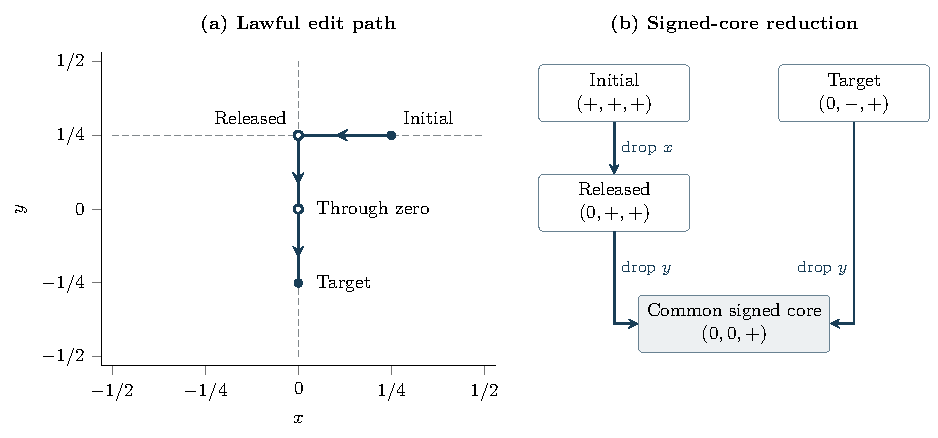
\includegraphics[width=\linewidth]{figures/signed_core_path.pdf}
 \caption{A lawful connection and its signed core at the same experimental
 profile. In (a), the dashed branches and the solid path together give
 the real lawful locus at \(z=1/4\) with the fourth response fixed at
 zero. The arrows trace the segments sampled by rational edits. The open
 circles are included intermediate states. In (b), the tuples give the
 signs of \(x,y,z\), and the arrows represent contractions. The initial
 law reaches the common signed core in two contractions and the target
 law reaches it in one. The calibration protects the positive sign at
 \(z\). Equality of the two signed cores is the reachability test at this
 fixed profile in \Cref{thm:native}.}
 \label{fig:staged-path}
\end{figure}

The support calculation behind this path is already instructive. A damping
weight specifies how many powers of a common parameter to multiply into each
response. As long as \(x,y,z\) are nonzero, the weight equations are
\(w_x+w_y=w_x+w_z\) and \(w_z=0\). They allow a contraction of \(x\) and force
\(y\) to survive. After \(x\) vanishes, the first equality is still true and
has zero on each side. It imposes no weight balance on the new support.
A second contraction can now remove \(y\). Both endpoints have the same signed
core, consisting of the positive calibrated \(z\). If the initial weight
equations were applied to every subsequent support, the initial positive
and target negative signs at \(y\) would stay distinct under all reductions.
This would incorrectly rule out \eqref{eq:opening-path}.

The geometric antecedent is the difference between a positive binomial
chart's closure and additional points of the full zero-allowing system.
Engstr\"om, Hersh and Sturmfels give an explicit example of that difference
in \emph{Toric Cubes}~\citep[Example~3]{toriccubes}.
The question here is whether such changes of active support admit a
\emph{complete} rational reachability criterion, and whether the criterion can
be recovered from actual held measurements. Sections~\ref{sec:spectral}
and~\ref{sec:native} address these two steps.

\subsection{Results and scope}

We first specify the measured model and the edit relation.
We then prove a separate theorem for bounded rational monomial systems.
It shows that a finite calculation on supports and signs captures every
real chart collision relevant to fine rational chains. The native theorem
combines it with homogeneous rate tests, conditional register constraints
and the order of attained profiles. The two complementary examples make
the criterion testable in both directions.

The lower-bound example uses the same coupled instrument for all six effects.
A subsequent classification of the available command families makes their
minimization precise. The terminal grade has a special role in the tests,
even when the command family takes the grade as an argument. We connect
these results to the witness predicates of Foundations~II in
\Cref{sec:witness-bridge}. The claims about reachability are specific to the
declared instruments, and the family count concerns the declared invocation
language.

\section{Audited Markov instruments and lawful edits}\label{sec:model}

\subsection{The native transition law}

Fix nonempty finite sets \(M,X,R\) of marks, base states and register cells.
The source state is \((g,u)\in X\times R\). Fix a finite family
\(\chi_i:X\to\{-1,1\}\), indexed by \(I\), with
\[
 \sum_{g\in X}\chi_i(g)=0,\qquad
 \sum_{g\in X}\chi_i(g)\chi_j(g)=|X|\,\mathbf 1_{i=j}.
\]
The nontrivial characters of a finite binary abelian group give examples,
and the proof uses only the displayed identities. Fix a mark reversal
\(m\mapsto\bar m\) of order at most two and a full-support rational
register law \(\nu\). A law consists of rational mark rates \(\theta_m\),
responses \(\alpha_{mi}\), and conditional register tables \(L_m(g,h;u,v)\).
Fix rational \(\delta>0\) and \(0\leq\kappa<1\).
Require
\begin{equation}\label{eq:guards}
 \theta_m\ge\delta,\quad \sum_m\theta_m=1,\qquad
 \sum_i|\alpha_{mi}|\le\kappa,\quad
 \alpha_{\bar m,i}=\alpha_{mi}.
\end{equation}
Write
\begin{equation}\label{eq:native}
 Q_m(g,h)=\frac{1+\sum_i\alpha_{mi}\chi_i(g)\chi_i(h)}{|X|},
 \qquad
 P_m((g,u),(h,v))=\theta_m Q_m(g,h)L_m(g,h;u,v).
\end{equation}
The tables \(L_m(g,h)\) have nonnegative entries, unit row sums and
stationary margin \(\nu\). Their reciprocal pairing is
\[
 \nu(u)L_m(g,h;u,v)=\nu(v)L_{\bar m}(h,g;v,u).
\]
There is one such table for each \(m,g,h\), so the register dynamics may
depend on the base transition.

The positive uniform term in \(Q_m\) has a probabilistic implementation.
Refresh the base uniformly with probability \(1-\sum_i|\alpha_{mi}|\).
With probability \(|\alpha_{mi}|\), choose a uniform endpoint with
\(\chi_i(h)=\sgn(\alpha_{mi})\chi_i(g)\), omitting zero-weight choices.
Balance gives exactly \eqref{eq:native}. In particular
\(Q_m(g,h)\ge(1-\kappa)/|X|>0\).
The unmarked kernel obtained by summing the marked entries is stationary
under \(\mu(g,u)=\nu(u)/|X|\). Indeed the conditional stationary margins
sum out the incoming register, after which the symmetric base kernel
preserves the uniform base law. The reciprocal identity is
\[
 \mu(g,u)P_m((g,u),(h,v))\,\theta_{\bar m}
 =
 \mu(h,v)P_{\bar m}((h,v),(g,u))\,\theta_m .
\]
This fixes the marked reversal relation even when the rates of reversed marks
differ.

\subsection{Held tests and their compiled equations}\label{sec:tests}

A timed word \(w\) is a nonempty finite sequence of marks of length at most
a fixed horizon. Let \(n_m(w)\) be the multiplicity of \(m\) in \(w\).
Its probability from a prepared state is
\(\pi_\theta(w)=\prod_m\theta_m^{n_m(w)}\).
After summation over the final register, its measured probability with
projected endpoint \(h\), from a preparation \((g,u)\), is
\begin{equation}\label{eq:word-return}
 \pi_\theta(w)\,(Q_{w_1}\cdots Q_{w_{|w|}})(g,h).
\end{equation}
This follows by iterative use of the register row sums. The base matrices
share the uniform projection and the orthogonal rank-one projections onto
the probes \(\chi_i\). Multiplying the base matrices multiplies the
eigenvalue on each probe, giving
\[
 \lambda_i(w)=\prod_m\alpha_{mi}^{n_m(w)}.
\]
These coordinates determine the word matrix, since the uniform term is
fixed and the other projections vanish on the orthogonal complement.

A \emph{license} names a comparison of two timed words of equal length.
The held comparison asks for equal word probabilities and equal conditional
projected endpoint laws. By \eqref{eq:word-return} it is also equivalent
to equality of the summed native word probabilities for all preparations
and all projected endpoints. Summing over endpoints recovers each
positive word mass, so the equality can be divided by that mass.
A fixed policy on subsets of the finite license catalogue specifies which
sets may be held.

The distinction between current and continuation tests also arises in
the study of predictive quotients for fixed-support route
transport~\citep{routeholonomy}. Here the licenses require specified
pairs of timed experiments to agree as the transition law changes.

A \emph{publication} is a named query with a stated rational value
that can be checked on the law. The catalogue consists of positive
word-mass ratios for equal-duration pairs and calibrations of the
form \(\alpha_{mi}=c\). For the latter, from any prepared native state
\((g,u)\),
\begin{equation}\label{eq:signal}
 \chi_i(g)\sum_{h,v} P_m((g,u),(h,v))\chi_i(h)=\theta_m\alpha_{mi}.
\end{equation}
This is a signed measurement. Dividing by the observed mark mass verifies the
calibration. Thus the held numerical tests on the rates are positive
homogeneous monomial equations, since the two degrees in a word comparison
equal the two lengths. The spectral tests are signed monomial equations on
\(\alpha\). They include the reversal equalities in \eqref{eq:guards}.
These two systems share the catalogue names and have separate numerical
variables.

\subsection{Capabilities and the edit relation}\label{sec:capabilities}

A profile \(p=(S,F,\Lambda,\mathcal A)\) records the positive native
proposal support \(S\), a schedule \(F=(F_0,\ldots,F_n)\) of partitions
of \(R\), the held licenses \(\Lambda\), and the publications \(\mathcal A\).
A decision at grade \(j\) is a function \(R\to\{0,1\}\) constant on the
classes of \(F_j\). As grades advance, the partitions may only refine.
For each available decision \(d\), require
\begin{equation}\label{eq:decision-mass}
 \sum_{v:\,d(v)=1} L_m(g,h;u,v)=\sum_{v:\,d(v)=1}\nu(v)
 \qquad\text{for all }m,g,h,u .
\end{equation}
These conditional tests are measured from the prepared transition table
because \(\theta_m Q_m(g,h)>0\). Equivalently it suffices to check
the terminal partition. Its block masses add to the masses of every
coarser disclosed block.

A state \(A\) is a profile \(p_A\) with a law that passes its tests,
has exactly its support, and respects the license policy. A profile is
\emph{attained} when some lawful rational state has that profile.
For profiles use the order
\begin{equation}\label{eq:profile-order}
 p\Refines q\quad\Longleftrightarrow\quad
 S_q\subseteq S_p,\quad
 F_j(q)\text{ refines }F_j(p)\text{ for all }j,\quad
 \Lambda_p\subseteq\Lambda_q,\quad \mathcal A_p\subseteq\mathcal A_q .
\end{equation}
The support is observable as the positive entries of \(P\). The
partitions are also observable from the available decisions.
Two cells lie in the same class precisely when every available
decision gives them the same value. Indicators of classes distinguish
different classes.

For a positive rational tolerance \(\varepsilon\), define elementary
edits on lawful states without using role labels. At fixed profile,
a local edit satisfies
\[
 \Norm{P_A-P_B}
 =\max_{m,s,t}|P^A_m(s,t)-P^B_m(s,t)|<\varepsilon .
\]
The other edits follow a cover of the finite order of attained profiles.
A cover is a strict increase with no attained profile strictly between
its endpoints. If the support is unchanged, the prepared transition
table stays fixed. If the support contracts, the projected marked
probabilities \(\theta_m Q_m(g,h)\) stay fixed. The conditional register may
change in that discrete edit. A chain means finite composition of
elementary edits, including the empty chain. We write \(A\leadsto_\varepsilon B\)
and call \(B\) \emph{factorable from \(A\)} if \(A\leadsto_\varepsilon B\)
for every positive rational \(\varepsilon\).

This definition keeps the numerical tolerance on the prepared law,
where it can be tested directly. Every step is directed in the
profile order, so an inherited license or publication remains held
at each later state.

\begin{theorem}[Audited Markov reachability]\label{thm:native}
Fix an instrument as above and let \(A,B\) be lawful rational states. Let
\(\SCore_{p_A}\) denote the signed core of \Cref{def:signed-core} for the
spectral equations compiled from the initial profile \(p_A\), including
the fixed reversal tests. Then
\[
 \bigl(\forall \varepsilon\in\QQ_{>0},\ A\leadsto_\varepsilon B\bigr)
 \quad\Longleftrightarrow\quad
 p_A\Refines p_B\quad\text{and}\quad
 \SCore_{p_A}(\alpha_A)=\SCore_{p_A}(\alpha_B).
\]
The criterion can be recovered from the measured experiments.
\end{theorem}

The next section gives the signed-core construction and proves its
rational completeness. Section~\ref{sec:native} proves the transfer
to native laws and capability changes.

\section{Rational reachability and the signed core}\label{sec:spectral}

Let \(J\) be a finite set of response coordinates. A held test has the form
\begin{equation}\label{eq:binomial}
 x^{u}=c x^{v},\qquad u,v\in\NN^J,\quad c\in\QQ,
 \qquad x^u=\prod_{j\in J}x_j^{u_j}.
\end{equation}
We use \(x_j^0=1\), including at \(x_j=0\). The guards are finitely many
absolute-sum budgets \(\sum_{j\in J_b}|x_j|\le b\), with rational
bounds and coordinate sets \(J_b\subseteq J\). Write
\(\mathcal F_{\QQ}\) for the lawful rational points. Assume that
\(\mathcal F_{\QQ}\) is bounded in \(\RR^J\). Covering \(J\) by
the budget sets suffices, as for the mark budgets in \eqref{eq:guards}.
The real lawful set is closed since the tests are polynomial equalities
and the guards are closed inequalities.
Two lawful rational points are \emph{finely connected} when for every
positive rational \(\varepsilon\) a finite chain in \(\mathcal F_{\QQ}\)
joins them with all successive sup-norm differences less than
\(\varepsilon\).

\subsection{Support reduction}

For a point \(x\), its \emph{signed chart} specifies \(S=\supp x\) and the
sign of \(x_j\) for every \(j\in S\). A row \((u,v)\) is active on \(S\)
when \(\supp u\cup\supp v\subseteq S\).
Let \(A_S\) be the matrix of row differences \(u-v\) for these active tests,
restricted to columns in \(S\).
On an inhabited chart, an active test has nonzero \(c\), compatible signs
and two nonzero monomials. An inactive test with nonzero \(c\) has
both monomials zero. A test with \(c=0\) requires its left monomial to vanish,
and this remains true on every smaller support. In the native class the
zero-coefficient case occurs only in a zero calibration.

\begin{definition}[Contraction and signed core]\label{def:signed-core}
Write \(S\to T\) if there are integer weights \(w_j\geq0\) on \(S\) such that
\[
  A_Sw=0,\qquad T=\{j\in S:w_j=0\}.
\]
A contraction keeps the signs on \(T\) and assigns zero off \(T\).
In a sequence of contractions use the matrix of the current support at
each step. Denote the least support reached from \(S\) by \(\Core(S)\)
and define
\[
 \SCore(x)_j=
 \begin{cases}
   \sgn(x_j), & j\in\Core(\supp x),\\
   0, & j\notin\Core(\supp x).
 \end{cases}
\]
The test list is fixed when constructing this map.
\end{definition}

\begin{lemma}[Realization and restriction]\label{lem:contraction}
A contraction on an inhabited rational signed chart can be realized
from every rational point of that chart by arbitrarily fine rational
chains with the indicated endpoint signs. Moreover, \(S\to T\)
restricts to \(U\to U\cap T\) for every \(U\subseteq S\).
The least reachable support in \Cref{def:signed-core} exists, is unique,
and is unchanged by further reductions.
\end{lemma}
\begin{proof}
For realization, let \(x\) be the initial rational point and set
\(x_j(t)=x_jt^{w_j}\) for \(j\in S\) and \(x_j(t)=0\) otherwise, on
\(0\le t\le1\), again with \(t^0=1\). For \(t>0\), equal total weights
preserve every active test and the inactive tests stay true. At \(t=0\)
the polynomial equalities hold by continuity. Absolute-sum budgets
can only decrease. The resulting curve is continuous, and its samples at
rational parameters are rational, including its limiting endpoint.
A sufficiently fine rational mesh gives the claimed chains.

For restriction, a row active on \(U\) was active on \(S\) and has no
factors outside \(U\). Cutting \(w\) down to \(U\) therefore preserves its
weight balance. The zero-weight coordinates in \(U\) are \(U\cap T\).
Repeated restriction gives the same intersection rule for an entire
reduction path.

Choose a reachable support \(C\) of minimum cardinality. For every reachable
\(U\), restrict the path from \(S\) to \(C\) to \(U\); this reaches
\(U\cap C\) from \(U\). Since \(U\cap C\) is also reachable from \(S\),
minimality forces \(C\subseteq U\). Thus \(C\) is least, is reachable from
every reachable support and is still least there.
\end{proof}

\paragraph{Finite calculation.}
For a prescribed survivor set \(T\), impose \(w_j=0\) on \(T\) and
\(w_j\ge1\) elsewhere on \(S\) in the rational linear system \(A_Sw=0\).
Clearing denominators produces an integer witness from any feasible
rational one. To compute the core, at each support test, for each \(j\),
whether the nonnegative balance system admits \(w_j\ge1\).
The sum of one witness for each feasible \(j\) removes the entire set of
currently removable coordinates in one step. Recompute the matrix and
repeat. Every nonempty round removes a coordinate, and a stable support
has no proper reduct. By \Cref{lem:contraction} it is the core.

\subsection{Limits of charts}\label{sec:chart-limits}

\begin{lemma}[A chart limit gives a contraction]\label{lem:limit}
If \(b\) lies in the real closure of a lawful signed chart on support
\(S\), then the chart contracts to \(\supp b\) with the signs of \(b\).
This holds even when the particular meeting point \(b\) is irrational.
\end{lemma}
\begin{proof}
Take a sequence \(x^{(k)}\) from the chart converging to \(b\).
Put \(T=\supp b\) and \(Z=S\setminus T\).
Surviving coordinates retain their signs by convergence.
If \(Z\) is empty, use zero weights. Otherwise, with
\(\ell^{(k)}=\log|x^{(k)}|\) on \(S\), the active equations are
\[
 A_{S,T}\ell^{(k)}_T+A_{S,Z}\ell^{(k)}_Z=\log|c|,
\]
where the right side lists the log-magnitudes of the active coefficients.
The vector \(\ell^{(k)}_T\) is bounded, while every entry of
\(\ell^{(k)}_Z\) tends to \(-\infty\). Hence
\(A_{S,Z}\ell^{(k)}_Z\) is bounded. Choose a linear right inverse
\(B\) on the image of \(A_{S,Z}\). The vectors
\[
 \ell^{(k)}_Z-B A_{S,Z}\ell^{(k)}_Z\in\ker A_{S,Z}
\]
are eventually strictly negative in every coordinate, because only a
bounded correction was subtracted. Negation gives a strictly positive
vector in the real kernel. The matrix has integer entries, so a rational
basis of its kernel and rational approximation give a positive rational
vector as well. Clear denominators and extend by zero on \(T\).
The resulting integer weights give precisely the required contraction.
\end{proof}

\subsection{Exact rational motion within a chart}\label{sec:rational-chart}

\begin{lemma}[Rational chart interpolation]\label{lem:rational-chart}
Any two lawful rational points of the same signed chart are finely connected
through rational points of that chart.
\end{lemma}
\begin{proof}
Fix endpoints \(x,y\) on support \(S\). Their real log segment has coordinates
\[
 \xi_j(t)=\sgn(x_j)|x_j|^{1-t}|y_j|^t \quad(j\in S)
\]
and is zero outside \(S\). It preserves the active equations, since their
log form is affine. Each absolute-sum budget is a convex function of the
log vector. At \(0<t<1\) a budget containing a changed coordinate has
strict slack, by strict convexity of the exponential in that coordinate.
Every unchanged block has exactly its endpoint values throughout.

To obtain rational samples that satisfy the equalities exactly, factor
each positive rational ratio
\(\rho_j=|y_j|/|x_j|\) as \(\prod_p p^{z_{jp}}\), with integer exponents
and a finite set of primes shared across the coordinates. The endpoints
satisfy the same active equations, so \(\rho^{u-v}=1\) for each active
row. Unique factorization gives \(A_S z_p=0\) for every vector \(z_p\)
of prime exponents. All \(z_{jp}\) vanish where \(\rho_j=1\).
At an interior time \(t\) choose positive rationals \(r_p\) close to \(p^t\).
The coordinates \(x_j\prod_p r_p^{z_{jp}}\) are rational, have the
required signs, and satisfy every exact test. Unchanged coordinates stay
fixed. The remaining inequalities hold when the choices are close enough
to the real segment, because those budgets have strict slack at \(t\).

By uniform continuity choose a finite mesh on the real segment with
successive differences less than \(\varepsilon/3\). Approximate each
interior sample within \(\varepsilon/3\) as above and use the given
rational endpoints. This gives all required successive differences.
\end{proof}

\begin{theorem}[Signed-core classification]\label{thm:spectral}
In the stated bounded class of held monomial systems, rational lawful
points \(x,y\) are finely connected if and only if \(\SCore(x)=\SCore(y)\).
\end{theorem}
\begin{proof}
For sufficiency, contract each endpoint to its core using
\Cref{lem:contraction}. Equality of signed cores puts the resulting rational
points in the same chart. Join them by \Cref{lem:rational-chart} and reverse
the chain from the second endpoint to its core.

For necessity, take the closure in \(\RR^J\) of the lawful rational
points in each chart they inhabit. There are finitely many such charts.
These closures are compact by the assumed bound and remain in the real
lawful set. If two of them meet, \Cref{lem:limit} contracts both charts
to the same signed support. By \Cref{lem:contraction}
they have the same signed core. Thus unions of chart closures for
different core values are disjoint compact sets. When there is more
than one value, their smallest pairwise distance is positive.
No rational chain of smaller mesh can cross from one such union to another,
and every lawful rational point belongs to its chart union.
This proves the necessary condition.
\end{proof}

The two uses of real analysis have separate returns. A real collision
determines a discrete support reduction. Real interpolation is then
sampled by rational points that obey the original equalities. The
reachability theorem is about finite chains at each tolerance, and in
particular does not require a continuous path taking only rational values.

\section{Transfer to native Markov edits}\label{sec:native}

\subsection{The structure of an attained cover}

\begin{proposition}[Effect types of elementary edits]\label{prop:effects}
Every elementary edit has exactly one of the effect types in
\Cref{tab:effects}. The types are determined by the named experiments.
\end{proposition}

\begin{table}[ht]
\centering
\small
\begin{tabularx}{\linewidth}{@{}lX@{}}
\toprule
Effect & Change in the experimental record\\
\midrule
Local rewrite & Vary the prepared law at fixed profile within the prescribed tolerance.\\
Gate & Contract support by a cover at fixed projected marked law.\\
Route & Advance the timed license catalogue by a cover at fixed law.\\
Earlier disclosure & Refine the available decision partition at one earlier grade by a cover at fixed law.\\
Terminal packaging & Refine the terminal decision partition by a cover at fixed law.\\
Publication & Advance the audit catalogue by a cover at fixed law.\\
\bottomrule
\end{tabularx}
\caption{The measured distinctions in the elementary edit relation.}
\label{tab:effects}
\end{table}

\begin{proof}
The fixed-profile case is the local rewrite. Now let \(p<q\) be an
attained cover and choose lawful laws at \(p\) and \(q\).
If their supports differ, use the register table from \(q\) at the
rates and spectrum of the law at \(p\), while keeping the old grades,
licenses and publications. The later register satisfies the old coarser
conditional decision tests. Rates and spectrum continue to pass their
old tests. This realizes the intermediate profile obtained by replacing
the old support alone with the new support. It lies strictly above \(p\).
The cover makes it equal to \(q\).

Suppose the support agrees. The later law can realize an advance in
licenses alone by taking the full license set of \(q\) and all other
fields of \(p\). The policy holds for that license set by attainment of
\(q\), even if the policy would deny some intermediate subsets.
An advance in publications alone is realized by the same later law
at the old license set. Thus if either catalogue differs, the
corresponding intermediate profile already equals \(q\). The update
may add several names when the cover skips unattained intermediate
sets.

In the remaining case only the grades differ. Advance the latest
differing grade to its value in \(q\). Earlier grades were coarser than the
old value at that grade, and every later grade already agrees with \(q\).
Nesting is therefore preserved. The later law realizes this profile
since each of its new decision partitions is no finer than that of \(q\).
The cover property again forces the intermediate profile to be \(q\).
The changed grade itself distinguishes the earlier and terminal cases.
All the cases are disjoint, and their tested fields are recoverable
from the experiments.
\end{proof}

\subsection{The metric return and the rate fiber}

Let \(N=|X\times R|\). Sum one prepared row of \(P_m\) to recover
\(\theta_m\). Use \eqref{eq:signal} to recover the response from the same
prepared row by dividing by \(\theta_m\).
If the native sup-norm difference between two laws is \(\eta\),
each of these two numerators changes by at most \(N\eta\), since
the signal weights are signs. A reference response has magnitude at
most one, and both rates are at least \(\delta\). Subtracting the
quotients gives
\begin{equation}\label{eq:inverse-modulus}
 \Norm{\alpha_A-\alpha_B}\le \frac{2N}{\delta}\,\eta .
\end{equation}
Conversely, the polynomial formulas \eqref{eq:native} are uniformly
continuous in the rates, responses and register entries on the
bounded boxes under consideration. One can use the bound on the
difference of three-factor products by the sum of their differences,
since \(\theta_m,Q_m,L_m\) all lie in \([0,1]\).
These observations connect numerical steps in both directions.

For use in the forward construction, the rate laws at a fixed
profile are finely connected. To see this, let \(\theta,\theta'\)
be two feasible rational rate vectors. If they agree, keep them fixed.
Otherwise take the componentwise geometric interpolation
\(\gamma_m(t)=\theta_m^{1-t}(\theta'_m)^t\) and normalize by
\(\sum_m\gamma_m(t)\). Homogeneity preserves every test after
normalization. Every numerator is at least \(\delta\).
For \(0<t<1\) the sum is strictly less than \(1\), by the
weighted arithmetic--geometric mean inequality and the fact that at
least one coordinate changed. All normalized rates are therefore
strictly above the floor for interior times. Use the prime-exponent
construction of \Cref{lem:rational-chart} for the positive endpoint
ratios, then normalize the rational interpolants. This keeps the tests
exact and works sufficiently close to every interior mesh point
because the floor has slack. The endpoints themselves are used
verbatim.

\subsection{Proof of native reachability}

\begin{proof}[Proof of \Cref{thm:native}]
For the forward direction, every elementary edit increases the profile
in \eqref{eq:profile-order} or keeps it fixed. Each later law therefore
passes all initially held spectral tests, and all discrete covers preserve
the spectrum. For any prescribed positive rational spectral mesh
\(\rho\), take a native chain at tolerance
\(\delta\rho/(2N+1)\). By \eqref{eq:inverse-modulus} its projected spectral
steps have size less than \(\rho\). \Cref{thm:spectral} then gives equality
of the signed cores relative to the initial tests.

For the converse assume profile comparability and equality of these
cores. Form the intermediate profile \(p'\) by taking the support
of the target profile and all other fields of the source. It is attained
by the target register at the source rates and spectrum. Between the
source profile and \(p'\), the other fields are fixed. Follow a finite
cover chain in that interval, selecting a register with the attained
support at each step and keeping the source rates and spectrum. These
are legal gates because the register constraints and held rate and spectral
constraints have separate variables.

At \(p'\) the current and target laws both meet the source's tests.
The two register tables have the same positive support. Their affine
interpolation preserves the prescribed margins, reciprocal pairing and
conditional block masses. It is positive exactly on that support, and a
rational mesh realizes its changes. Keeping the final register fixed, move
the rates by the preceding rate argument and move the spectrum by
\Cref{thm:spectral}, both with the source's tests held. The three numerical
chains can use a small enough mesh to meet the given native tolerance
by \eqref{eq:native}. At this stage the target law is attained with profile
\(p'\). Follow a finite cover chain from \(p'\) to the target profile
while keeping that law fixed. Every intermediate attained profile has
the target support and weaker tests. Its license policy holds because
the profile is attained. This makes each step legal and yields the
requested chain for every positive rational native tolerance.
\end{proof}

\begin{proposition}[Readback of edits]\label{prop:readback}
For a fixed instrument, the prepared probabilities and the named
decision, license and publication responses determine the state.
The correspondence with attained query tables preserves and reflects
elementary edits, effect types and finite chains, including chains with
a specified effect omitted. A relabeling that identifies the full
attained profile order and the named queries gives the same conclusion
for the relabeled instrument.
\end{proposition}
\begin{proof}
The positive entries give the support, and the available decisions give each
partition by their common equality relation. Catalogue membership is read
from the remaining queries. The prepared probabilities determine rates and
spectra by the preceding row-sum and signal calculations. Finally
\[
 L_m(g,h;u,v)=\frac{P_m((g,u),(h,v))}{\theta_m Q_m(g,h)}
\]
recovers every register entry. The denominator is strictly positive by
\eqref{eq:guards}. Thus attained states and their attained query tables
correspond in both directions. The fixed-profile comparison, cover order and
law or projected-law preservation in the edit definition can all be tested
on the tables. The same tests define the edits after relabeling when
the relabeling identifies the attained order and the experiment labels,
including the terminal grade. Lifting each step in a finite chain proves
the claim.
\end{proof}

\section{Connection, obstruction and the six effects}\label{sec:two-examples}

We use the same small carrier for the two contrasting reachability
examples and the family count. Take \(X=\{0,1\}\) with its single
nonconstant parity probe and \(R=\{0,1,2,3\}\) with uniform mass.
The four marks have rate \(1/4\) and each reverses to itself.
Take \(\delta=1/8\), \(\kappa=1/2\), horizon two and two grades.
Let \(F_*\) denote the split \(\{0,1\}\mid\{2,3\}\).

The reset register has all entries \(1/4\). The gated register differs
only for one designated mark and the base pair \(g=h=0\). In that
conditional table replace its \(\{0,1\}\)-by-\(\{0,1\}\) submatrix by
\[
 \begin{pmatrix} 1/2 & 0\\ 0&1/2\end{pmatrix}.
\]
Both tables have the required stationary margins and reciprocity.
The conditional mass of each block of \(F_*\) is \(1/2\) for every
preparation in either table. The gated table is genuinely coupled to
the base pair, and loses precisely the two reciprocal proposals
between cells \(0\) and \(1\) at the designated mark and base pair.

\subsection{An exact edit through two zero responses}\label{sec:staged}

For the example of \Cref{sec:opening-example}, use the gated register
at the third mark. Hold the split at both grades, the route equality
between the first--second and first--third words, and the calibration
\(z=1/4\). Fix the fourth response at zero. Every point of
\eqref{eq:opening-path} is a lawful spectrum. Along the first segment
\(y=1/4\); along the last two \(x=0\).
The original route equality and all other tests therefore hold.

For an affine segment with varying response from \(a\) to \(b\),
choose an integer \(D>|b-a|/\varepsilon\) with \(D\ge1\) and sample
\(a+(b-a)k/D\) for \(0\le k\le D\). The difference in each marked
entry is bounded by the magnitude of the varying response change,
by the explicit two-state formula and the fixed rate and register.
The resulting rational edits are strictly within \(\varepsilon\).
The projected probability of retaining the parity bit at the
second mark changes from \(5/8\) to \(3/8\), conditional on the mark.
The prepared, marked contributions to these probabilities are
\(5/32\) and \(3/32\), respectively.
Throughout this construction the native support is fixed, since
\(Q_m>0\) and the register has the same support.

The held calibration requires \(w_z=0\) on every support containing
\(z\), and the reversal rows are identities. On
\(\{x,y,z\}\), the held word requires \(w_y=w_z\).
It follows that a single contraction cannot reach the core
\(\{z\}\), and that a surviving \(y\) keeps its positive sign.
The legal successive contractions remove \(x\) and then \(y\).
On the target support \(\{y,z\}\) the same second contraction
removes the negative \(y\). Thus both signed cores have the value
\(+1\) at \(z\) and zero elsewhere.
A rule that keeps the initial weight balances at all later supports
forces \(w_y=0\) at every step. Every reduct of each endpoint would
retain its different sign at \(y\). No common signed reduct is possible
under that frozen rule. This failure occurs even though the original
word probabilities are equal throughout the explicit chain.

\subsection{A pair that requires all six effects}\label{sec:omissions}

For a second catalogue on the same carrier, name the marks
\(a,b,c,d\) and let the initial responses be
\((1/4,1/4,-1/8,1/8)\).
Initially use the reset register and the indiscrete partition at both
grades. Hold the route \(aa\sim bb\) and the calibration
\(\alpha_b=1/4\). The optional license compares \(ca\) with \(da\),
and the optional publication checks \(\alpha_c=1/8\).
Both are defined in the fixed catalogues. All license subsets are
allowed by policy.

Construct the following chain of changes. Each row describes the
change from the state already attained by the preceding rows.
\begin{table}[ht]
\centering
\small
\begin{tabularx}{\linewidth}{@{}lXX@{}}
\toprule
Effect & Realizing change & Observable that forces the effect\\
\midrule
\(P_2\) & Gate the conditional register at mark \(c\) and base pair \(0,0\). &
Two reciprocal positive native proposals disappear.\\
\(P_1\) & Move \(\alpha_c\) from \(-1/8\) to \(1/8\) through zero. &
The measured \(c\)-response changes.\\
\(P_5\) & Disclose \(F_*\) at grade \(1\). &
The terminal decision becomes available.\\
\(P_4\) & Disclose \(F_*\) at grade \(0\). &
The earlier decision becomes available.\\
\(P_3\) & Add the license \(ca\sim da\). &
The named timed comparison is held.\\
\(P_6\) & Publish the calibration \(\alpha_c=1/8\). &
The named measurement can be cited.\\
\bottomrule
\end{tabularx}
\caption{One sequence of changes on the coupled carrier. Each adjacent pair has a lawful chain at every positive tolerance.}
\label{tab:omissions}
\end{table}
The gate is a cover, since reciprocity requires the two deleted
proposals to be removed together. The change of \(\alpha_c\) is
an affine move at fixed profile while no held numerical test
constrains that coordinate. It has arbitrary rational meshes.
Each partition advance is a cover, since nothing lies between the
indiscrete partition and a partition into two given blocks along
this refinement. Each catalogue change adds one name.
The new license passes because the \(c\) and \(d\) responses
agree by then and all the mark rates agree. The new publication
is exactly the measured \(c\)-response.

\begin{theorem}[Six measurable effects on one carrier]\label{thm:omission}
For each of the six effects there is an adjacent pair in
\Cref{tab:omissions} connected at every positive rational tolerance
whose connection requires that effect. Moreover the same initial
and final states of the entire table are connected at every positive
rational tolerance, and every connecting chain uses all six effects.
These statements also hold on the attained experimental readouts.
\end{theorem}
\begin{proof}
The preceding construction establishes connection. Every step of
another type preserves the listed observable in the third column.
For \(P_1\), this is the measured response, which all discrete steps
preserve even when a gate changes the conditional register.
For \(P_4\), no other type changes any earlier grade.
For \(P_5\), the observable is terminal availability.
The other three exclusions follow from support, the license set,
and the publication set, respectively. Thus each failure persists
under composition. The endpoints of the entire table differ in
all six listed observables, so all six types are required in every
connection. Readback follows from \Cref{prop:readback}.
\end{proof}

\subsection{A positive-tolerance obstruction}\label{sec:obstruction}

Use the initial profile of the second example and replace only
\(\alpha_a=1/4\) by \(-1/4\). Both endpoint laws pass the same held
tests. Their common calibration pins \(b\) at \(1/4\) and their
route equality forces \(\alpha_a^2=\alpha_b^2\). Thus \(w_b=0\)
and \(2w_a=2w_b\) on the occupied supports, so the respective
opposite signs of \(a\) survive. In particular the signed cores
differ. The obstruction is also quantitative. Each intermediate
law must pass the original route and calibration, hence its
\(a\)-response belongs to \(\{1/4,-1/4\}\). With \(N=8\) and
\(\delta=1/8\), a rewrite at tolerance
\[
 \frac{\delta(1/2)}{2N+1}=\frac1{272}
\]
has response change less than \(1/2\) by \eqref{eq:inverse-modulus}.
A discrete step fixes the response. Therefore no chain at this
positive tolerance can cross the two branches.
This contrasts with the earlier example in which a zero
response changes the active damping system without invalidating
the held tests.

\section{The minimum number of command families}\label{sec:basis}

An \emph{edit position} here is a writable part of the measured
record. For a numerical edit it is the local-law position.
For a discrete edit it is the support, the schedule entry at one
given grade, the license catalogue, or the publication catalogue.
The existence and uniqueness of the position follow from the cover
argument and the named readouts. A single invocation at a grade
overwrites that grade's decision entry and leaves every other
entry fixed. It still must be a legal cover between attained states.

\begin{definition}[Single-write families]
A family offers all lawful instances of one command with a fixed
mutation mode and a fixed writable field. A command for the
decision schedule has one grade argument whose domain is fixed
independently of the state and tolerance. It offers a single grade
write at each allowed argument. The four nonclock command modes
offer local-law edits, gates, route licenses and publications,
respectively. A catalogue is \emph{complete} at a tolerance if it
generates the full chain relation at that tolerance. It is a
\emph{basis} if it is complete and deleting any family destroys
completeness.
\end{definition}

\begin{lemma}[Live positions]\label{lem:live}
Call a position live at a positive tolerance if some nonidentity
elementary edit there is lawful. A catalogue is complete exactly
when it offers every live position. It is a basis exactly when
it offers all live positions and each family has a live position
offered by no other family.
\end{lemma}
\begin{proof}
Coverage is sufficient because each nonidentity elementary step
can be invoked at its position. Identity steps may be replaced
by the empty chain. For necessity, choose a live witness at an
omitted position. If it is the support, one grade, or one of the
catalogues, all other positions preserve that field, so that witness
cannot be realized. For a nonidentity local-law edit, the two
profiles agree. In any alternative chain between them, monotonicity
of support prevents a strict gate. With the local-law position
also omitted, every remaining edit fixes the law. The local
witness is again impossible. Apply the coverage test after deleting
each family to obtain the last characterization.
\end{proof}

\begin{theorem}[Five families and the terminal split]\label{thm:basis}
One uniform grade-indexed family together with the four nonclock
families offers the same elementary relation as the earlier--terminal
split, for every instrument in the class and every tolerance.
On the coupled two-grade instrument of \Cref{sec:omissions}, at
every positive rational tolerance, there are exactly two irredundant
catalogues in the declared language. These are the uniform
five-family catalogue and the split six-family catalogue.
The uniform five-family catalogue is the unique minimum-size
complete catalogue there. Five is the minimum number sufficient
for the entire class in this language.

If a successful invocation's family name alone must determine
whether it changes the terminal decision readout, the split
catalogue is the unique irredundant catalogue satisfying that
contract on the two-grade instrument.
\end{theorem}
\begin{proof}
The uniform grade family offers a decision write at every grade.
In the split catalogue the same invocation is offered by the
earlier family or by the terminal family according to its grade.
This is a bijection of invocations preserving the grade,
measured endpoints, and legality. Every finite chain is
therefore preserved.

On the coupled example all six positions are live at every
positive tolerance. The discrete examples are covers.
The response rewrite supplies a nonidentity step at every
positive tolerance by subdivision.
\Cref{lem:live} forces the four nonclock modes and coverage
of both grade positions. A family offering both grades makes
any other grade family redundant. If there is no such family,
the two singleton domains are necessary. The resulting two
catalogues are irredundant by their private live positions.
This proves the classification and the lower bound. The uniform
construction realizes that bound class-wide.

In the split catalogue every family name specifies whether the
terminal decision changes. The two live writes at the two
grades in the uniform family have different answers to that test.
The uniform catalogue therefore fails the added contract.
The classification leaves the split catalogue as the unique
irredundant one satisfying it on this instrument.
\end{proof}

There are six independently witnessed effects in
\Cref{thm:omission} and five families in the specified minimum.
Two grade-specific effects share one invocation rule while remaining
distinct measurements. The additional contract places that
distinction in the family name itself.

\section{Realizing the Foundations II witnesses}\label{sec:witness-bridge}

Foundations~II fixes witness predicates \(W_1,\ldots,W_6\), together
with record closure, audit honesty and requirements on active role
projections~\citep[Sections 2, 4 and 5]{foundations2v3}. We use the
selected positive alternatives described below to connect the roles
to the experiments of \Cref{sec:omissions}.

\begin{proposition}[Witness realization on the coupled instrument]\label{prop:witness-realization}
The coupled instrument admits one finite audited typed description
with an active projection for each of the six Foundations~II roles.
Each projection uses a witness tied to the measured change in the
corresponding row of \Cref{tab:omissions}. The two attained query
tables in that row are connected at every positive rational
tolerance, and every such connection uses the corresponding effect.
\end{proposition}

\begin{proof}
Use one description containing the prepared-law snapshots in
\Cref{tab:omissions} and the records for the six finite checks. We
describe each selected witness condition and check it on the data
that change in the associated edit.

\paragraph{\(W_1\). Descent of an updated native law.}
Use a uniform preparation token with a mark, an index in
\(\{0,\ldots,15\}\) and an index in \(\{0,\ldots,3\}\).
The mark is the output mark. The base stays if the first index is
below the count for that mark and flips otherwise. The counts are
\((10,10,7,9)\) before the rewrite and \((10,10,9,9)\) after it. The second
index selects the next register. At the gated mark and base pair,
if both the prepared cell and drawn index belong to \(\{0,1\}\),
the output retains the prepared register.
This finite experiment has exactly the prepared probabilities,
including the deleted entries.
At the updated law the fixed token \((c,7,0)\) gives a total
update, grouping preparations by base and output records by mark
and base. Equal-base preparations in cells \(0\) and \(1\) give a
nontrivial source class. Every pair in a source class has equal
output mark and base, so the updated map descends to that
readout. The earlier law gives a different base output for the
same token and prepared base. This is the same \(c\)-response
change used in the rewrite omission witness.

\paragraph{\(W_2\). Loss of a realizer at the gate.}
Use the full domain of positive native proposals after the gate
as the candidate class for the map from proposals to destinations.
The specification is equality with the erased proposal from
cell \(0\) to \(1\) at the gated mark and base pair.
Its truth table is false throughout the candidate class and
true on the recorded same-kind erased proposal, which was
positive at the old law. The universal check and the empty
satisfying list certify the no-realizer alternative.

\paragraph{\(W_3\). Parallel words and the complete rule list.}
Use the reached word summaries of length at most two, with one
overflow state. Each summary contains elapsed time, word mass
and conditional parity response. At the disclosed law \(ca\)
and \(da\) give paths with the same start and finish.
The recorded source rule is \(aa\sim bb\). In the two-element OR
monoid send \(c\) to \(1\) and the other marks to \(0\).
The two sides of the old rule agree, while \(ca\) and \(da\)
differ. The comparison survives every contextual application
of the recorded rule and witnesses separation under the
complete source rule list. The later license admits precisely
this comparison. Before the rewrite their parity responses
were different.

\paragraph{\(W_4\) and \(W_5\). Earlier access and the terminal quotient.}
For \(W_4\), the ordered grades at which the block decision is
available grow from \(\{1\}\) to \(\{0,1\}\). The restricted strict
order is irreflexive and transitive, and has a strict pair only
after earlier disclosure.
The \(W_5\) witness uses the terminal map \(u\mapsto\mathbf 1_{u<2}\)
on the full register. Its graph gives the exact kernel, a merged
pair and a reached range. The terminal edit makes the bit
available at grade \(1\) with grade \(0\) fixed. The earlier edit
discloses it at grade \(0\) with the terminal reading fixed.

\paragraph{\(W_6\). Replay of a published calibration.}
The evaluator at the licensed law has a loaded state and
two absorbing answers. It computes the signed native signal
and compares it to the mark mass times \(1/8\). The accepted
trace has two entries and an exact check of the evaluation
step. A separate conformance check ties the evaluator to the
prepared table. The earlier gated law fails the same query.
The ordinary execution and conformance claims have first-layer
audits before the role audit records \(W_6\).
The edit adds the citeable receipt at fixed law.

The content checks evaluate the formulas on the full declared
domains, including the false evaluations and the universal
no-realizer check for \(W_2\). Role claims target the same
clusters as their thresholds, witness annotations, levels and
scope annotations. Their audited premises include the
recomputed positive witness check. This supplies the selected
positive \(W_i\) and active projections on one description.
The finite witness description contains the snapshots used by
the six checks. The reachability and omission assertions on their
attained query tables are those of \Cref{thm:omission}, transported
by \Cref{prop:readback}.
\end{proof}

\section{Relation to the foundations program and prior work}\label{sec:discussion}

\subsection{What the experimental result establishes}

The operational result gives three different answers on one class.
\Cref{thm:native} decides reachability between laws. \Cref{thm:omission}
decides which observable effects cannot be removed from the language
of a given connection. \Cref{thm:basis} measures how the same
elementary edits can be grouped into command families. The distinctions
are recoverable from named experiments, and the operational theorem
is invariant under presentations of the same instrument that preserve
those experiments and the attained profile order.

These results give a model of a layer that can be revised while
preserving its source commitments. A route equality already held can
still pass when its local restrictions on future changes weaken.
Admitting a new test is a separate change from a numerical step made
to satisfy it. A decision can become available earlier without a
change in the terminal package, and two grade-specific effects can
be implemented by the same rule. These are the concrete uses of
the role vocabulary in this instrument.

Foundations~II describes six typed witness channels over finite audited
typed closure descriptions (\Fatcd{}). Its general upper bound
assumes recognition, and the six channel slots are part of the
description scheme~\citep[Theorem 9.1]{foundations2v3}.
Foundations~III classifies typed interactions between those roles under
a fixed audit instrument~\citep{foundations3}.
\Cref{prop:witness-realization} gives the exact witness connection for
one coupled model. This provides semantic and operational content
for the six modeled roles, while the abstract recognition question
retains its own hypotheses. In particular, the present operational
upper bound classifies the elementary edits of
\Cref{sec:capabilities}.

\subsection{Binomial geometry and components}

The closest geometric comparison is \emph{Toric Cubes}. In one
inhabited signed chart with source \(x\), write a coordinatewise
damping ratio \(0<u_j\le1\) and put \(w_j=-\log u_j\).
Its positive domain is given by \(A_S w=0,\ w\ge0\).
The guards remain valid under such damping. Each equality is
two binomial inequalities in \(u\), so the closure of this
source-relative positive damping domain is a toric cube.
Engstr\"om, Hersh and Sturmfels give its monomial parametrization
and the compatible boundary cell structure~\citep[Lemma 1 and
Theorems 1--2]{toriccubes}. Their Example~3 also illustrates why
the full binomial system can include boundary points beyond the
positive closure. The use of monomial damping in a fixed support
and the weakening of consequences when factors vanish both
have this antecedent.

The full lawful set in \Cref{thm:spectral} ranges over
different signed charts, with a new balance system at each smaller
support. Its classification uses the restriction property across
these systems, the detection of all chart collisions by contractions,
and exact rational interpolation under guards. Cellular and Laurent
binomial decompositions~\citep{eisenbudsturmfels}, support theory for
nonnegative exponential-family closures~\citep{geigermeeksturmfels,rauhkahleay},
and signed gluing in real toric varieties~\citep{sottile,soprunovasottile}
supply earlier forms of these geometric ingredients. General algorithms
already compute real semialgebraic components~\citep{basupollackroy}.
The signed-core result gives a direct invariant of the held rows
for exact rational fine chains, together with a native stochastic return.
Termination and joinability also have the classical rewriting
antecedent of Newman~\citep{newman}. In the Six Birds treatment of
rewriting, joinability of elementary branches is formulated as local
flatness~\citep{sixbirdsconfluence}. Here the joinability argument uses
the fact that one contraction restricts to a smaller support by
intersection even after some rows cease to be active.

The Fourier computation for group-based Markov models is
classical~\citep[Section 2 and Theorem 6]{sturmfelssullivant}, as is
the block-sum criterion for lumpability~\citep[Theorem 6.3.2]{kemenysnell}.
The present model uses named timed word experiments and signed
calibrations to impose exact equations on laws that can themselves
be edited. Its reachability question concerns those laws.
In algebraic statistics, Markov bases connect nonnegative integer
tables at fixed linear sufficient statistics~\citep[Theorem 3.1]{diaconissturmfels}.
That discrete move problem has its own binomial interpretation.
The law variables, permitted steps and size quantifiers here are
different.

\subsection{Edit effects and readout sufficiency}

Rodgers's \emph{Lawhood Necessity} distinguishes four exclusion roles
from the three operators that implement them~\citep[Theorem 3.1 and
Remarks 3.1 and 5.1]{rodgerslawhood}. The analogous distinction here
is between the six observable effects and the five command families
that generate the same lawful edit chains. Rodgers also derives
a criterion for when an observation coordinate is indispensable
for a given family of relations~\citep[Theorems 5.1 and 6.2]{rodgerscompletion}
and shows that strong marked quotients preserve adaptive transcript
laws under substitution in matching causal
contexts~\citep[Theorems 6.1--6.2]{rodgersboundaries}. These results
concern which distinctions a readout must retain. In \Cref{thm:native},
the held experiments constrain the changes of the underlying law.

Nadendla's six typed epistemic morphisms give a further
comparison. The strongly admissible traces in that calculus
have an exact normal form ordered by an explicit phase and
a tacit phase~\citep[Definition 2 and Theorem 17]{nadendla}.
The typing and the classified objects differ from those in the
native edit language. The common number does not provide a
translation between the two systems.

\subsection{Scope of the probability model}

The refresh guard does substantive work. Strict positivity of a
general kernel does not ensure that shrinking independent spectral
magnitudes preserves its positivity. For an example on the binary
group of order four, take the three nontrivial Fourier responses
\((4/5,4/5,7/10)\) in the order of two generators and their
product. The four row numerators are
\(33/10,3/10,3/10,1/10\), all positive. Holding the first two
responses fixed while damping the third to zero gives the
negative numerator \(-3/5\) at the displacement on which
both generators are negative. In the instrument of \Cref{sec:model},
each mark's absolute-sum budget gives a coordinatewise
downward-closed region. This is why the contraction curve
can be used as a physical edit.

The proof also uses equal durations in the rate tests, which
make normalization compatible with the equations, and a strict
rate floor for the inverse metric estimate.
The forward capability argument uses the separation of
conditional register constraints from rate and spectral constraints.
These hypotheses define the present result. Extensions to other
preparation laws or different test families would have to replace
the corresponding links in the proof.

The restriction to individual word probabilities also limits the
equations the tests can impose. With fixed projected kernels, the held
word tests give a conformal normal form and a row-space criterion
for invariant affinities (\Cref{thm:fixed-normal-form,thm:fixed-affinity}).
An equality between probabilities of two finite events of the same
duration can impose any rational polynomial equality on the rate
simplex. Already on a one-state instrument it can isolate any
prescribed finite number of lawful rational rates at the same profile.
Below a positive native tolerance, no lawful chain joins two of
those laws, even with a common strict rate floor
(\Cref{thm:finite-event}).

\appendix
\section{Mechanization and reproducibility}\label{sec:mechanization}

The Lean project is in \path{lean}.
Its root is \path{MovingProjection.lean}.
The table lists declarations relative to the
\path{MovingProjection} namespace.

\begin{center}
\small
\begin{tabularx}{\linewidth}{@{}>{\raggedright\arraybackslash}p{0.34\linewidth}>{\raggedright\arraybackslash}X@{}}
\toprule
Paper result & Lean declarations\\
\midrule
Least support and chart limits &
\path{exists_core}, \path{IsCore.unique}, \path{contracts_of_limit}\\
Rational spectral classification &
\path{fineConnected_iff_signedCore}\\
Timed probabilities and native reachability &
\path{NativeExperiments.licensed_trajectory_test},\newline
\path{NativeExperiments.published_calibration},\newline
\path{NativeExperiments.exact_six_iff}\\
Effects and table readback &
\path{NativeExperiments.elementary_iff_unique_effect},\newline
\path{NativeExperiments.same_tests_same_effect},\newline
\path{NativeExperiments.table_exact_six}\\
Common witness and obstruction &
\path{Example.single_edit_requires_all_six},\newline
\path{Example.obstructionTolerance_value},\newline
\path{Example.obstruction_at_native_tolerance}\\
Clock families and terminal contract &
\path{Example.every_basis_two_grades},\newline
\path{Example.minimum_complete_catalogue},\newline
\path{Example.six_with_terminal_contract}\\
Recomputed and frozen damping &
\path{StagedContraction.edits_through_zero},\newline
\path{StagedContraction.no_single_contraction_to_core},\newline
\path{StagedContraction.signed_cores},\newline
\path{StagedContraction.frozen_rejects}\\
Foundations II witnesses on the coupled description &
\path{Example.Manuscript.all_roles_active},\newline
\path{Example.Manuscript.role_realization},\newline
\path{Example.Manuscript.one_recorded_edit_needs_all_six}\\
\bottomrule
\end{tabularx}
\end{center}

Run \verb|lake build| from \path{lean} with Lean and Mathlib v4.28.0.
The project includes the Foundations~II role and raw-record
definitions used by the witness bridge in \path{lean/SixBirds}.
The checked least-support definition chooses a least reduct
classically after proving it exists and is unique.
The finite feasibility procedure in \Cref{sec:spectral} is a
mathematical algorithm for the support.
The correspondence table in Foundations~II documents the separate
schema projection status of its general recognition-relative
theorem~\citep[Appendix B]{foundations2v3}.
The declarations above implement the native results and the
particular witness bridge.
The fixed-projection normal form, affinity criterion and finite-event
result in \Cref{sec:companion} have written proofs in the appendix.
Their statements are outside the scope of this Lean correspondence.

\section{Fixed-projection edits and finite-event tests}\label{sec:companion}

This appendix gives three results about the choice of instrument and
tests. With fixed projected kernels, a conformal normal form factors
edits by conditional-flux circuits and prime-valuation moves. The
held tests determine precisely which rate ratios and cycle
affinities~\citep{schnakenberg} are invariant. Allowing finite-event comparisons gives a separate
obstruction to fine reachability, even with a single native state.

\subsection{A conformal normal form at fixed projection}

Fix a finite native state space \(X\), a positive rational stationary
distribution \(\mu\), a finite set \(M\) of marks with an involution
\(m\mapsto\bar m\), and a surjection \(b:X\to B\) onto a finite set.
For each mark fix a rational stochastic matrix \(Q_m\) on \(B\).
A native law has positive rational rates \(\theta_m\) summing to one
and rational conditional stochastic kernels \(K_m\) on \(X\). Its
marked transition probabilities are \(P_m(x,y)=\theta_m K_m(x,y)\). Set
\(C_m(x,y)=\mu(x)K_m(x,y)\) and require
\begin{equation}\label{eq:fixed-flux}
 C_{\bar m}=C_m^{\mathsf T},\qquad
 \sum_{y:\,b(y)=v}C_m(x,y)=\mu(x)Q_m(b(x),v).
\end{equation}
The transpose condition makes both margins of every \(C_m\) equal to
\(\mu\). A positive marked edge has stationary flux ratio
\begin{equation}\label{eq:fixed-flux-ratio}
 \frac{\mu(x)P_m(x,y)}{\mu(y)P_{\bar m}(y,x)}
 =\frac{\theta_m}{\theta_{\bar m}}.
\end{equation}
The prepared marked rows recover \(\theta_m\) by summation and recover
\(C_m\) by division and multiplication by \(\mu(x)\).

A profile records the positive marked support, a nested schedule of
partitions \(F_0,\ldots,F_T\) of \(X\) with fixed initial partition
\(F_0\), a route license, and a set of citeable checks from a fixed
finite catalogue. At step \(t\) the probability of each mark and next
block of \(F_{t+1}\) must be constant on each current block of \(F_t\),
a stepwise lumpability condition; compare the block-sum
criterion~\citep[Theorem 6.3.2]{kemenysnell}.
Decisions at grade \(t\) are binary functions on the blocks of \(F_t\).
The route license is a congruence on the monoid of mark words up to
a fixed length, with an absorbing overflow element. An identified
pair must have equal length, equal probability, and equal conditional
projected endpoint laws. A live check specifies a positive rational
ratio of probabilities of two words of equal length. Each law
holding the check supplies an exact executed replay bound to that
law. Historical checks refer to immutable source records.
Profiles are attained if some lawful rational law
realizes them. The order on attained profiles contracts support,
refines partitions, and enlarges the congruence and check set.

Let \(H_F\) be the subspace of \(L^2(\mu)\) of functions constant on
the blocks of \(F\). The stepwise disclosure tests are equivalent to
\begin{equation}\label{eq:fixed-terminal}
 K_m H_{F_T}\subseteq H_{F_0}\qquad(m\in M).
\end{equation}
Indeed, the stepwise conditions are \(K_m H_{F_{t+1}}\subseteq H_{F_t}\).
By nesting, \(H_{F_t}\) is invariant under every \(K_m\) for \(t<T\).
Since \(K_m^*=K_{\bar m}\) by \eqref{eq:fixed-flux}, its orthogonal
complement is also invariant. Hence \(K_m\) annihilates
\(H_{F_{t+1}}\cap H_{F_t}^{\perp}\). Summing these orthogonal increments
gives \eqref{eq:fixed-terminal}, which in turn implies each stepwise
condition by nesting. The observed marked paths preserve the full
stationary path-reversal likelihood ratio. The micro path ratio is
the product of \eqref{eq:fixed-flux-ratio} over its marks, hence is
constant on each observed path class. Summing over that class gives
the same ratio against the reversed path with reversed observation
schedule and marks.

For a word \(w\) with count vector \(a(w)\), its probability from any
preparation is \(\theta^{a(w)}\) and its conditional projected kernel
is the product of the \(Q_m\) in word order. Equal summaries stay
equal in common contexts by multiplication of probabilities and
kernels, and equal lengths overflow together. Thus on an attained
profile the nontrivial rate constraints from the licenses and live
checks have the form
\begin{equation}\label{eq:fixed-rate-rows}
 \theta^{d_i}=c_i,\qquad
 d_i\in\mathbb Z^M,\quad \sum_{m\in M}(d_i)_m=0,\quad c_i\in\QQ_{>0}.
\end{equation}
Write \(D\) for their exponent matrix. The conditional-flux tests
are rational affine equations by \eqref{eq:fixed-flux} and
\eqref{eq:fixed-terminal}, with positivity on the profile support
and zero elsewhere. The law fiber therefore separates into
conditional-flux and rate factors.

An elementary capability edit is a cover of attained profiles.
A support cover keeps the rates fixed, and the other covers keep
the full law fixed. Numerical edits hold the profile fixed. For
fluxes, irreducible numerical directions are circuits of the
homogeneous equations on the fixed support, meaning nonzero
directions of inclusion-minimal support, with collinear
subdivisions counted as one direction. These are the flux changes
that admit no noncollinear conformal splitting, the elementary vectors
of Rockafellar~\citep{rockafellar}. For rates, use
the additive coordinates
\(v_p(\theta_m/\theta_n)\) for primes \(p\) and ordered pairs
\((m,n)\), where \(v_p\) is the prime exponent of a positive
rational. An irreducible rate change is supported at one prime and
its difference cannot be split into two nonzero lawful differences
conformal to it. A difference is conformal to another if each
nonzero entry has the same sign and no greater magnitude. The
irreducible rate changes at a prime are thus the Graver basis
elements of the lattice of lawful prime-exponent displacements~\citep{graver}.

\begin{theorem}[Fixed-projection normal form]\label{thm:fixed-normal-form}
Two lawful rational endpoints are connected by these edits exactly
when their profiles are ordered in the direction of the edit.
The capability covers each change a single capability. Disclosure
covers split one block at one grade, route covers adjoin one pair
and take congruence closure, and publication covers add one check.
Together with the numerical changes, the effects are the six
in \Cref{tab:effects}, distinguished by the same fields and clock
grades. Test-preserving relabelings preserve the effect types and
the elementary numerical directions.
\end{theorem}

\begin{proof}
For a feasible support contraction from \(C\) to a retained mask
\(N\), optimize over the closed polytope of conditional-flux tables
\(Z\) satisfying the old affine tests and vanishing off \(N\).
Maximize \(\eta\geq0\) with \(Z_e\geq\eta C_e\) for every \(e\in N\).
A feasible table positive on \(N\) implies a positive optimum.
The objective is bounded by \(|M|/\sum_{e\in N}C_e\), and a rational
vertex attains it. On its optimal face minimize
\(\sum_{e\in N}(Z_e-C_e)^2/C_e\). On the smallest face containing
the minimizer, the affine equations of the face and the linear
gradient conditions along its tangent space have rational
coefficients. They determine the minimizer uniquely by strict
convexity, hence it is rational. Its support is \(N\). Keeping the
rates fixed preserves every old rate test.

At a fixed profile let \(u\) be the target conditional-flux
displacement. Choose a rational homogeneous direction \(v\ne0\)
with signs compatible with \(u\), supported in \(\supp u\), and
with inclusion-minimal support among such choices. If a nonzero
homogeneous direction were supported on a proper subset of
\(\supp v\), one could add a rational multiple in one of its two
directions up to the first zero of \(v\), keeping the signs and
leaving a nonzero result. This contradicts minimality. Thus \(v\)
is a circuit. The direction space on its support is one-dimensional
because two independent directions on that support would have a
nonzero linear combination canceling a coordinate. Thus any
conformal splitting of a circuit is collinear. Scale \(v\) by
\(\min_{e\in\supp v}|u_e/v_e|\) and subtract that step from the
residual \(u\). At least one more entry is at its target and every
entry stays between its original and final values. The affine
tests and positivity on the support are preserved. For a
displacement of nonminimal support the first step is supported on
a proper subset of \(\supp u\), giving a noncollinear splitting.
Iteration terminates because the residual support strictly decreases.

For the rate factor, a pair of lawful rate vectors
\(\theta,\widehat\theta\) has
\(z_p(m)=v_p(\widehat\theta_m/\theta_m)\) in \(\ker D\) at each prime,
by unique factorization in \eqref{eq:fixed-rate-rows}. Only finitely
many primes occur. The possible displacements at a prime are the
integer lattice
\[
 \{(z_m-z_n)_{m,n\in M}:z\in\mathbb Z^M,\ Dz=0\}.
\]
Choose a nonzero lattice element of least \(\ell^1\)-norm among
those conformal to the residual at that prime. It is irreducible,
since any conformal splitting would give a smaller such element.
Subtract and repeat until the integer norm is zero. The element
with lift \(z\) is realized by
\begin{equation}\label{eq:fixed-prime-move}
 \theta'_m=\frac{\theta_m p^{z_m}}{\sum_{n\in M}\theta_n p^{z_n}}.
\end{equation}
Normalization cancels in the homogeneous tests and pairwise rate
ratios. This jump changes only the prescribed prime
in the ratio coordinates. Matching all pairwise ratios gives the
target normalized rates.

If the endpoint profiles are ordered, the target law also attains
the profile with the target mask and the source's other fields.
This follows from block summation in \eqref{eq:fixed-terminal} and
inclusion of the held tests. Every support-changing cover therefore
changes only the support. If the support agrees, the upper law
attains each intermediate choice of nested partitions, congruence
and checks between the two profiles. Thus a cover can change only
one of those fields. Among different grades, advancing the latest
differing one preserves nesting. Its blocks can be split one at a
time into two unions of upper blocks, so a cover makes just one
binary split. For a congruence cover, adjoining any new pair and
taking its congruence closure stays below the upper congruence.
The cover forces equality. A check cover adds one name.

Take successive support covers first, preserving the earlier tests.
Apply the circuit and prime decompositions on the final mask, then
take the remaining capability covers at the final law. The attained
order is finite and the numerical decompositions terminate. Every
allowed step is monotone in the profile order, proving the converse.
The readouts recover the masks, partitions, congruences, inventories,
conditional fluxes and rate ratios used in these tests. Relabeling
preserves the homogeneous spaces and support of flux differences,
and permutes the pairwise rate coordinates, so it preserves the
elementary numerical directions and capability effects. The example
below supplies the joint lower bound.
\end{proof}

\paragraph{A coupled edit with a changing affinity.}
Take \(B=\mathbb Z/4\) and \(X=B\times\{0,1,2,3\}\) with uniform
\(\mu\). The marks \(+,-,c,h\) translate the base by \(1,-1,2,0\),
respectively, with \(+\) and \(-\) reversed and the other marks
self-reversing. Initially every conditional register table resets
uniformly and the partitions at grades \(0,1,2\) are indiscrete.
Use the length-two route horizon. Normalize the initial rate weights
\((4,1,3,2)\), hold \(+-\sim hh\), and hold
\(\theta_c/\theta_-=3\). Both licensed words have zero displacement
and equal probability, and all nonempty contexts for them overflow.

At base point \(0\) for mark \(h\), delete the two register
transitions between \(0\) and \(1\) and add the deleted entries to
the two corresponding diagonals. This is a support cover because
the deleted proposals form one reversal pair. For the rational
gate in the proof, untouched rows bound the optimum by \(\eta=1\).
The stated table attains this bound. At equality the row and
column sums leave only the indicated diagonal increases. In the
clockwise table from base point \(0\), change the conditional register fluxes at
\((0,2),(1,3),(0,3),(1,2)\) by
\((1,1,-1,-1)/32\), with transposed changes in its reverse table.
Here conditional register flux uses the uniform register weight
\(1/4\). The zero-margin space on these entries and their reverses
is one-dimensional and any nonzero direction uses all of them.
This is a circuit and makes the register law depend on base position.

Apply \eqref{eq:fixed-prime-move} with lifts \((-2,0,0,-1)\) at
\(2\) and \((2,0,0,1)\) at \(3\). The successive rate weights are
proportional to \((1,1,3,1)\) and \((9,1,3,3)\). The equations
\(\theta_+\theta_-=\theta_h^2\) and \(\theta_c/\theta_-=3\) hold
throughout. The relative lattice has rank one and each move
changes \(v_p(\theta_h/\theta_-)\) by one in magnitude, so both are
irreducible. The clockwise four-cycle affinity changes from \(4^4\)
to \(9^4\).

\subsection{Which affinities the held tests determine}

\begin{theorem}[Affinity row-space criterion]\label{thm:fixed-affinity}
At a fixed attained profile, a zero-sum integer exponent
\(d\in\mathbb Z^M\) gives an invariant relative monomial
\(\theta^d\) under lawful numerical edits exactly when \(d\) is in
the rational row space of \(D\). Outside that space an exact rational
edit chain starting at any lawful rate vector changes \(\theta^d\).
The real rate fiber in the open positive simplex is smooth of
dimension \(|M|-1-\operatorname{rank}D\). For a fixed supported
closed marked walk, its multiplicative affinity is the monomial
with \(d=\sum_j(e_{m_j}-e_{\bar m_j})\).
\end{theorem}

\begin{proof}
The centered log coordinates
\(u_m=\log\theta_m-|M|^{-1}\sum_n\log\theta_n\)
identify the open positive simplex with the zero-sum hyperplane.
The inverse exponentiates and normalizes. The held equations are
\(Du=\log c\), with all rows in the zero-sum hyperplane, giving the
dimension. A row combination makes \(d\cdot u\) constant. Otherwise
rational elimination and clearing denominators give an integer
\(z\) with \(Dz=0\) and \(d\cdot z\ne0\). For any prime \(p\),
\eqref{eq:fixed-prime-move} preserves the held equations and changes
the monomial by \(p^{d\cdot z}\). The normal form realizes this
change by lawful rational numerical steps with the conditional
tables fixed. Multiplying \eqref{eq:fixed-flux-ratio} along the walk
gives the affinity formula.
\end{proof}

In the real fixed-profile fiber the rate factors are connected by
centered log segments and the conditional-flux factors by affine
segments on the fixed support. The proof below changes the permitted
probability tests and exhibits fixed profiles with isolated laws.

\subsection{Finite-event comparisons and failure of locality}

\begin{theorem}[Finite-event expressivity]\label{thm:finite-event}
For every rational polynomial on a positive rate simplex there are
two fixed events of the same finite duration in a one-state marked
Markov instrument whose probabilities agree exactly on the
polynomial's zero set. In particular, for any \(k\geq2\) one such
test gives a fixed-profile real law fiber consisting of exactly
\(k\) isolated rational laws. Below a positive native tolerance,
no numerical edit chain connects distinct laws in this fiber.
\end{theorem}

\begin{proof}
Clear denominators and homogenize to degree \(d\) using
\(\sum_m\theta_m=1\). The polynomial on the simplex is then
\(\sum_a n_a\theta^a\) for integers \(n_a\). Use a one-state
instrument with independent marks of rates \(\theta_m\), all
self-reversing. A constant truth value can be realized with two
identical events or with an empty and a full event, including on
a one-point simplex.

For at least two marks, choose distinct \(i,j\) and an integer
\(r\geq1\) with \(\binom{2r}{r}\geq\max_a |n_a|\).
There are that many words containing \(r\) copies each of \(i,j\),
all of probability \((\theta_i\theta_j)^r\). For each \(a\) with
\(n_a\ne0\), choose one length-\(d\) prefix with multiplicities \(a\)
and append \(|n_a|\) distinct such suffixes. The resulting words
are all distinct and have length \(d+2r\). Put the words for
positive coefficients in one event and those for negative
coefficients in the other. Their probability difference is
\[
 (\theta_i\theta_j)^r\sum_a n_a\theta^a.
\]
The prefactor is strictly positive. Common prefix and suffix
contexts multiply both event probabilities by the same factor
by independence, so the comparison also supports substitution
in those contexts.

With two rates \(t,1-t\), take the polynomial
\(\prod_{i=1}^k(t-a_i)\) for distinct rational
\(a_i\in(0,1)\). The support, disclosure schedule and held test
are identical at the \(k\) resulting laws. They are all the lawful
rates at this profile. The least distance \(\min_{i\ne j}|a_i-a_j|\)
in the native probability metric is positive, so smaller steps
cannot move between them. The same construction works under a
common rate floor \(0<\delta<1/2\) by choosing the roots in
\((\delta,1-\delta)\).
\end{proof}


\bibliographystyle{plainnat}
\bibliography{references}
\end{document}
